\documentclass[xcolor={dvipsnames},pdf, hyperref={colorlinks=true, citecolor=ForestGreen, linkcolor=BlueViolet, urlcolor=Magenta}]{beamer}
\usetheme{Frankfurt}  
\usecolortheme{whale}
\usepackage{tikz} 
\usepackage{amsmath}
\usepackage{amsthm}
\usepackage{amssymb}              % used for \eqref{} in this document
\usepackage{dsfont}
\usepackage{hyperref}
\usepackage{threeparttable}
\usepackage{multirow}
\graphicspath{{Figures/}}
\usepackage{booktabs}
\usepackage{tikz}
\newtheorem{exmp}{Example}[section]
\usepackage{subcaption}
\usepackage{adjustbox}
\usepackage{graphicx}
\usepackage[mathscr]{euscript}
\usepackage{remreset}% tiny package containing just the \@removefromreset command
\makeatletter
\@removefromreset{subsection}{section}
\makeatother
\setcounter{subsection}{1}
\usepackage{float}
\usepackage{sgamevar}
\usepackage{sgame}

\newcommand{\defn}[1]{\textbf{#1}}


%Instructor version
\newcommand{\blank}[0]{}
\newcommand{\ddp}[1]{{\textcolor{ForestGreen}{#1}}} 
\newcommand{\dd}[1]{{\underline{\textcolor{ForestGreen}{#1}}}}

%Student version
%\newcommand{\blank}[0]{\vspace{2em}}
%\newcommand{\dd}[1]{\underline{\hspace{3cm}}} 
%\newcommand{\ddp}[1]{}

\addtobeamertemplate{navigation symbols}{}{%
	\usebeamerfont{footline}%
	\usebeamercolor[fg]{footline}%
	\hspace{1em}%
	\insertframenumber/\inserttotalframenumber
}


\section{Externalities}

%% preamble
\title{Market Failure}
\author{David A. D\'iaz}
\institute{UNC Chapel Hill}
\date{}

\AtBeginSection[] %Section links on slides

\begin{document} 
	
	\begin{frame}
		
		\titlepage
		
	\end{frame}
	

\begin{frame}{Externalities}
	
	\begin{itemize}
		\item \textbf{Principle 7: Governments Can Sometimes Improve Market Outcomes}
		\item The purpose of this section is to see why markets sometimes fail to allocate resources efficiently and how government policies can improve such allocations.
		\item \defn{Externality:} The uncompensated impact of one agent's \textit{actions} on the well-being of a bystander.
	\end{itemize}
	
\end{frame}	

\begin{frame}{Externalities}
\begin{itemize}
		\item Externalities can have adverse effects (\dd{negative}) or beneficial impacts (\dd{positive}).
		\item Because buyers and sellers do not take into account the external effects of their actions, the market equilibrium is \dd{inefficient} when there are externalities.
		\item In the presence of an externality, society's interest extends beyond the well-being of market participants. 
\end{itemize}
\end{frame}

\begin{frame}{Negative Externalities}
\begin{itemize}
	\item The idea behind negative externalities is that there is some \dd{external cost} is not taken into account. 
	\item There is some \dd{private cost} of producing, while the cost to society is referred to as the \dd{social cost}. 
	\item The cost to society is given by \dd{private cost + external cost}.
	\item The social-cost curve is \dd{above} the supply curve because it takes into account the external costs imposed on society.
\end{itemize}
\end{frame}


\begin{frame}[b]{Negative Externalities}
\begin{figure}[H]
			\centering
			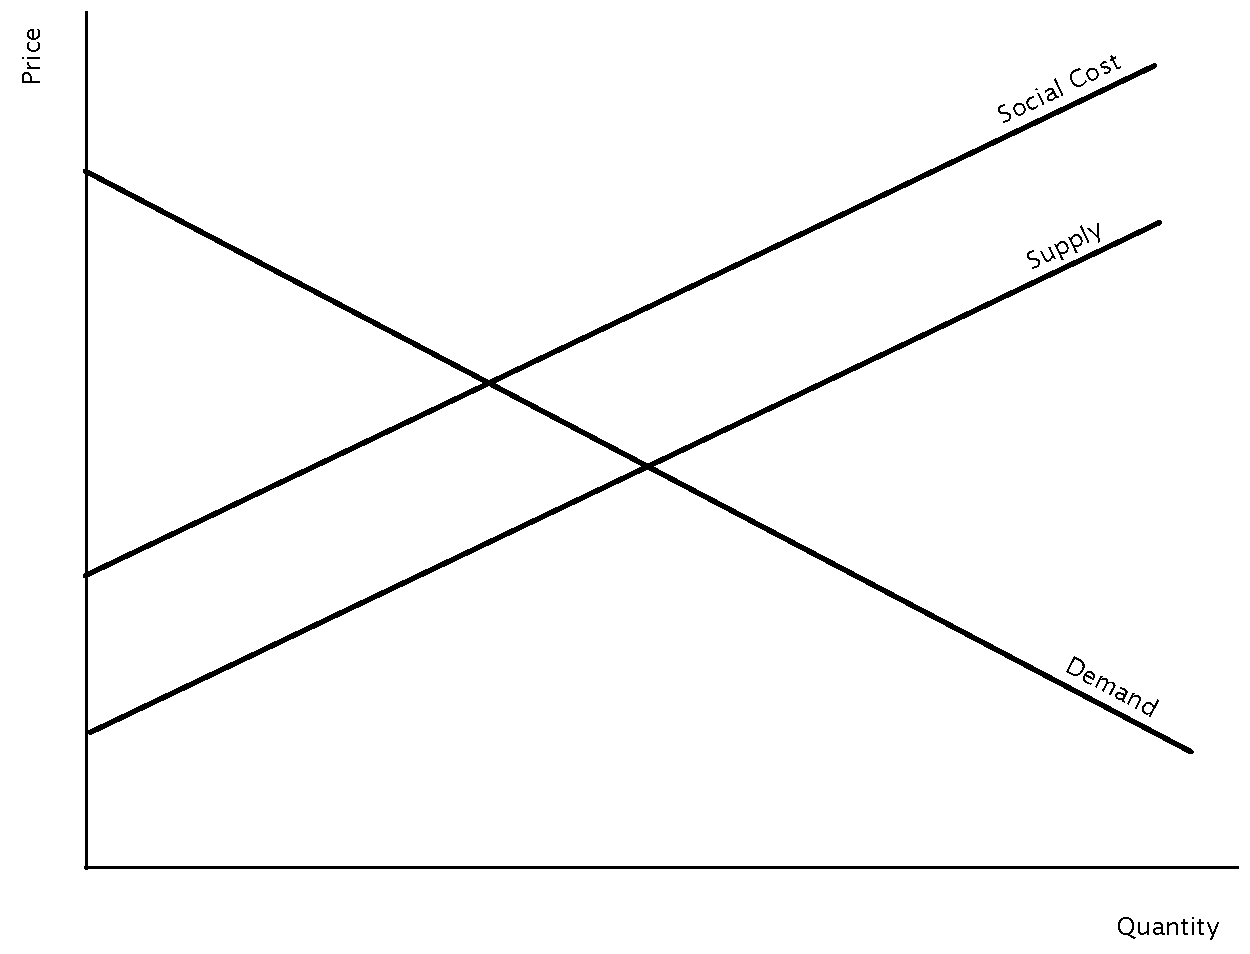
\includegraphics[scale=.35]{plot50.pdf}
			\caption{Negative Externality}
		\end{figure}

\end{frame}

\begin{frame}[b]{Negative Externalities}	
		\begin{figure}[H]
			\centering
			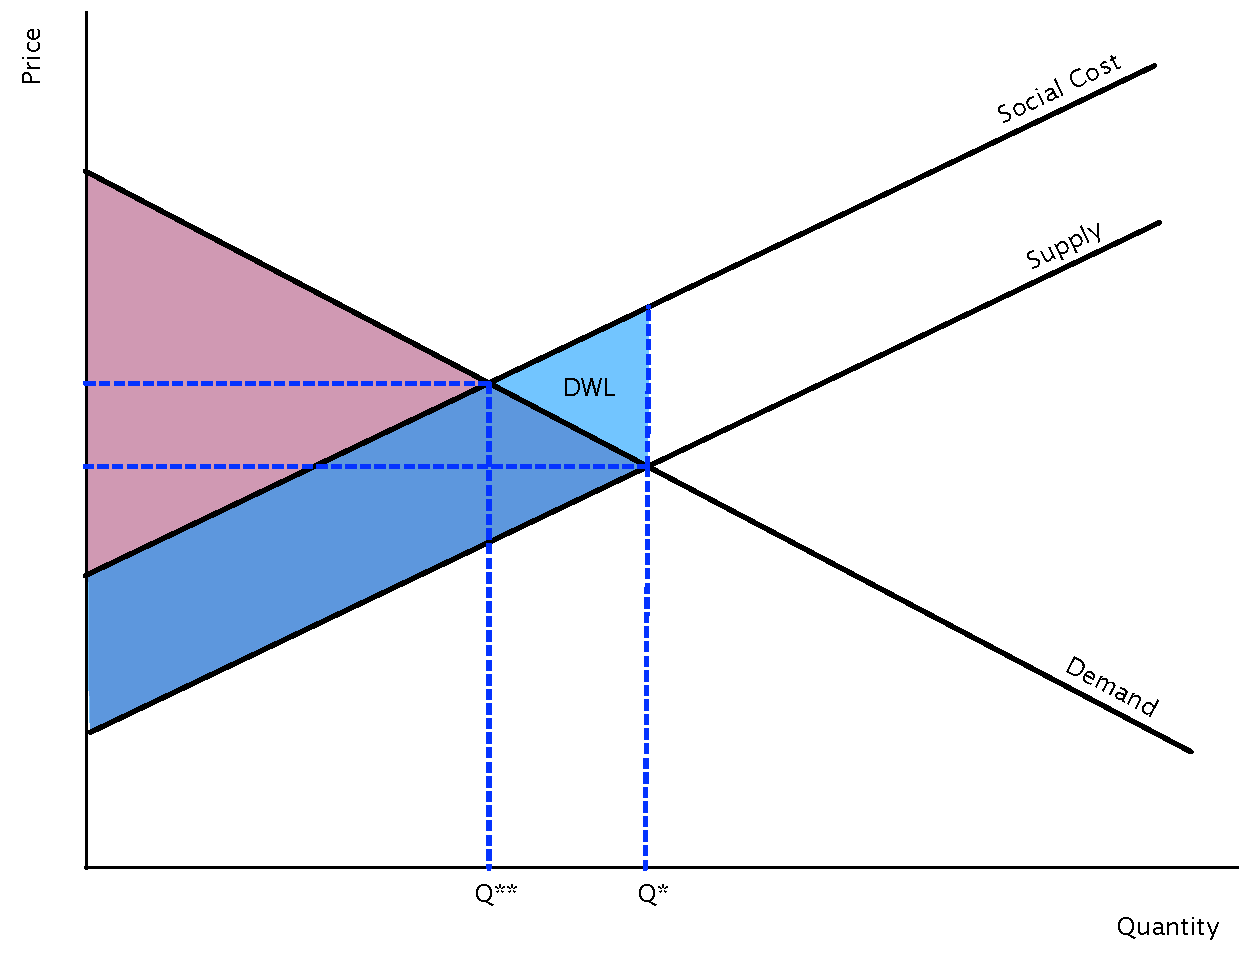
\includegraphics[scale=.35]{plot51.pdf}
			\caption{Negative Externalities and Welfare}
		\end{figure}
\end{frame}

\begin{frame}{Negative Externalities}
	\begin{itemize}
		\item 	We see that the optimum amount produced is given by the intersection of the \dd{social cost curve} and the \dd{demand curve}. 
		\item At quantities below $Q^{**}$, the value to consumers is \dd{greater} than the social cost
		\item  At quantities above $Q^{**}$ and below $Q^*$, the value to consumers is \dd{less} than the social cost.
		\item Thus, with a negative externality we have that the market equilibrium quantity produced is \dd{greater} than the socially optimal quantity. 
	\end{itemize}
\end{frame}

\begin{frame}{Negative Externalities}
	\begin{exmp} 
		\scriptsize
			Refer to Figure \ref{fig4}. What is the per-unit external cost? The total external cost at the market equilibrium? What is total surplus at the market equilibrium? The deadweight loss? What is the efficient quantity in this market?
		\end{exmp}
	
			\begin{figure}[ht!]
		\centering
		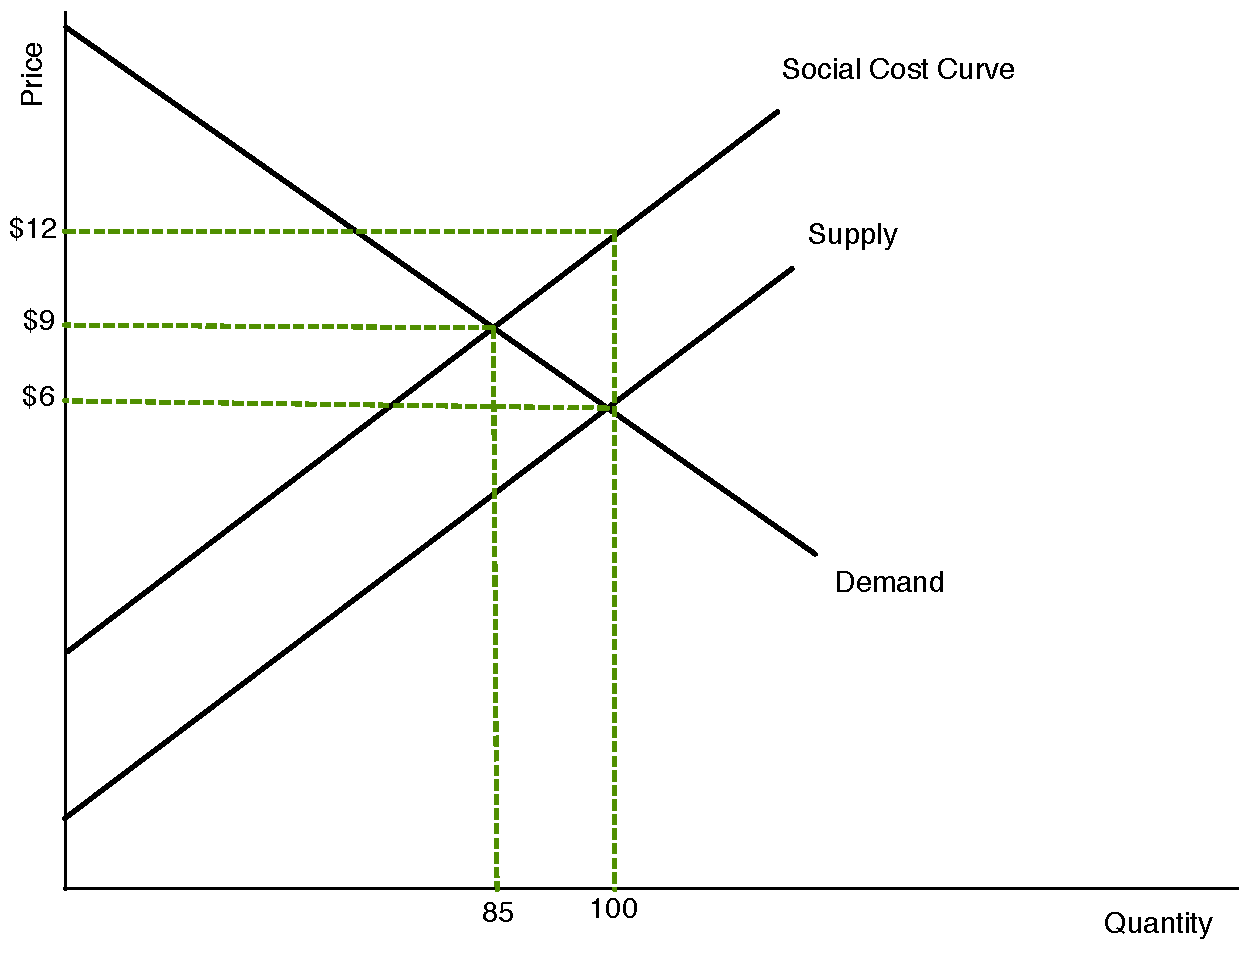
\includegraphics[scale=.30]{notes06_plot1.pdf}
		\caption{Market for Floor Cleaner}
		\label{fig4}
	\end{figure}


\end{frame}

\begin{frame}{Positive Externalities}
	\begin{itemize}
		\item 	On the other hand, some actions yield benefits to third parties. In cases such as this, we have positive externalities.
		\item In this case, there is some value that people partaking in an activity receive (\dd{private value}).
		\item Society as whole, however, also gets some \dd{external benefit} from this activity. The sum of these values is referred to as the \dd{social value}. 
	\end{itemize}
\end{frame}

\begin{frame}[b]{Positive Externalities}

	\begin{figure}[H]
		\centering
		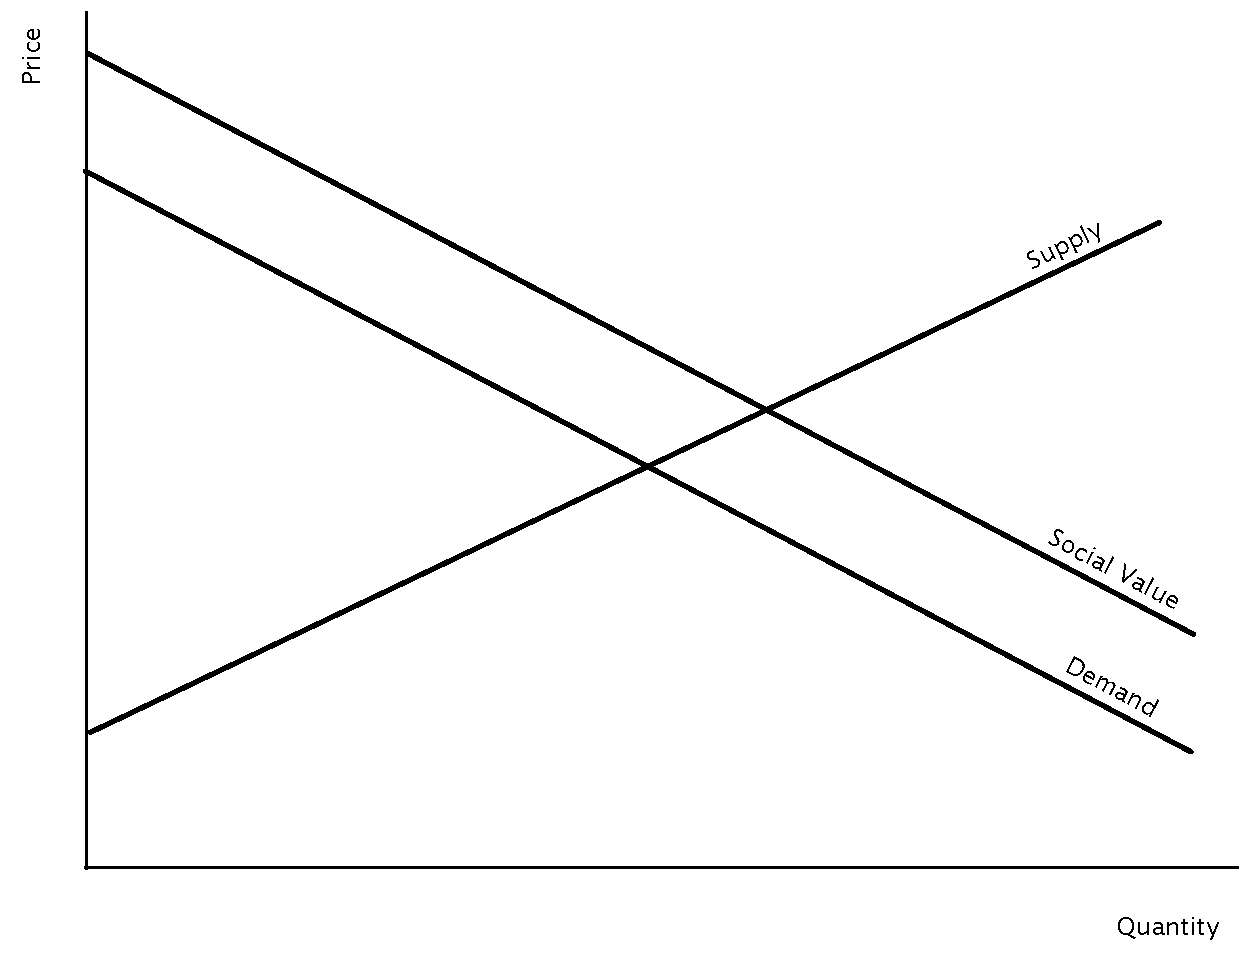
\includegraphics[scale=.35]{plot52.pdf}
		\caption{Positive Externality}
	\end{figure}
\end{frame}

\begin{frame}[b]{Positive Externalities}
		\begin{figure}[H]
			\centering
			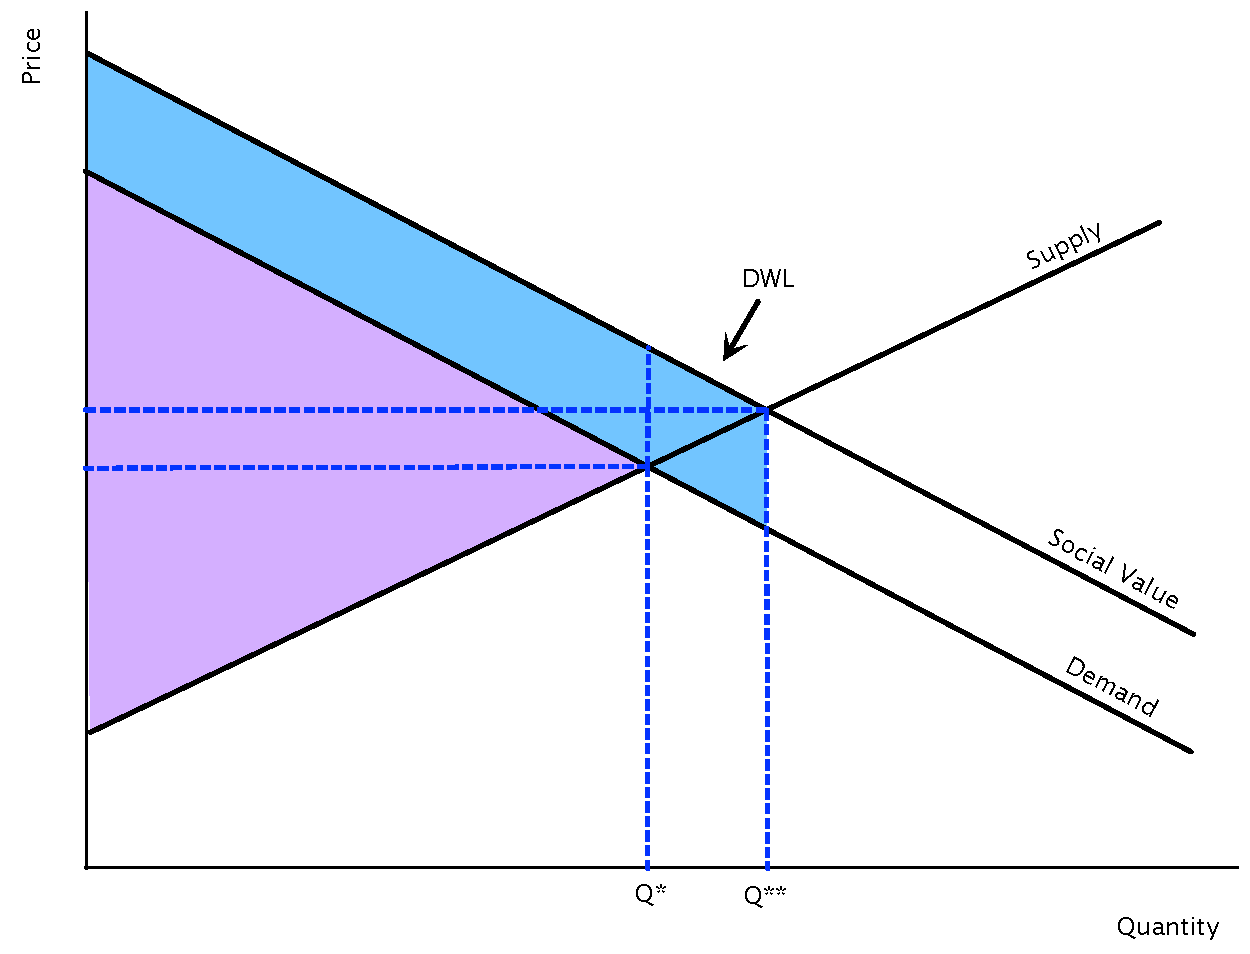
\includegraphics[scale=.35]{plot53.pdf}
			\caption{Positive Externalities and Welfare}
		\end{figure}
\end{frame}


\begin{frame}{Positive Externalities}
	\begin{itemize}
		\item 	Just like with a negative externality, the equilibrium market quantity is \dd{inefficient} in the presence of a positive externality.
		\item The optimum amount produced is given by the intersection of the \dd{social value curve} and the \dd{supply curve}. 
		\item For all quantities below $Q^{**}$, the social value is \dd{greater} than the private cost.
		\item Thus, with a positive externality we have that the market equilibrium quantity produced is \dd{less} than the social optimal quantity. 
	\end{itemize}
\end{frame}

\section{Correcting Externalities}

\begin{frame}{Correcting Externalities}
	\begin{itemize}
		\item If the presence of externalities distorts markets and makes them inefficient, how can the government (or private parties) correct this?
	
	\end{itemize}
\end{frame}



\begin{frame}{Correcting Externalities}
\begin{itemize}
	\item Public policies
	\begin{enumerate}
		\item Solution 1: Command \& control policies (i.e., regulation)
		\item Solution 2: Corrective tax or subsidy
		\begin{itemize} 
			\item To align private costs (values) with social costs (values), the per-unit tax (subsidy) must be equal to the \dd{per-unit external cost (benefit)}.
		\end{itemize}
		\item Solution 3: Tradable permits - create markets to trade rights to engage in some activity.
	\end{enumerate}
\end{itemize}
	
	
\end{frame}

\begin{frame}{Correcting Externalities}
	
\begin{itemize}
	\item Private solutions:
	\begin{enumerate}
		\item Moral codes and sanctions \ddp{(e.g., littering, public nudity)}
		\item Charities \ddp{(e.g., alumni donations)}
		\item Business integration \ddp{(e.g., bar and music venue)}
		\item Contracts \ddp{(e.g., outdoor concert hall and bar)}
	\end{enumerate}
\end{itemize}
\end{frame}

\begin{frame}{Correcting Externalities}
\begin{exmp} 
	\scriptsize
	There are two firms in Candyland, and each one pollutes as shown in Table \ref{pollution}.
	
	\begin{table}[H]
		\caption{Pollution by Firms in Candy Land}
		\label{pollution}
		\centering
		\begin{tabular}{ c|c|c}        
			
			Firm   & Initial Pollution Level  & Cost of Reducing Pollution (per unit)\\
			\hline
			Lolly LLC & 425 units & \$15 \\
			Gloppy Inc. & 300 units & \$10 \\
		\end{tabular}
	\end{table} 
	The government wishes to reduce pollution by 400 units and mandates each firm reduce their pollution level by 200 units. How much is each firm polluting now? What is the total cost of reducing pollution in this case?
\end{exmp}
\pause \scriptsize	\ddp{Lolly reduces pollution by 200 units. Cost = \$15 $\times$ 200 = \$3,000. \\
	Gloppy reduces pollution by 200 units. Cost = \$10 $\times$ 200 = \$2,000. \\
	Total pollution = $\underbrace{225}_{\text{Lolly}}$ + $\underbrace{100}_{\text{Gloppy}}$ = 325 units. Total cost = \$5,000.}
\end{frame}

\begin{frame}{Correcting Externalities}
\begin{exmp}
	\scriptsize
Instead, the government gives Lolly 200 pollution permits and Gloppy 125 permits that they can trade with each other. The firms decide to set a price of \$12/permit. How much would each firm pollute? What would be the total cost of reducing pollution?
\end{exmp}
\pause \scriptsize \ddp{Lolly will buy all the permits from Gloppy (high-cost polluter buys from low-cost polluter). Lolly will have 325 permits, Gloppy will have 0. \\
	Lolly: \\
	Buys 125 permits. Cost of permits = \$12 $\times$ 125 = \$1,500. \\ Able to pollute 325 units, but still has to reduce pollution by 100 units.\\ Cost of reducing pollution = \$15 $\times$  100 =\$1,500. Total cost to Lolly = \$3,000. \\
	Gloppy: \\
	Sells 125 permits. Revenue = \$12 $\times$ 125 = \$1,500. \\
	Has 0 permits, so must reduce pollution by 300 units. 
	\\Cost of reducing pollution = \$10 $\times$ 300 = \$3,000. Net cost to Gloppy = \$3,000 - \$1,500 = \$1,500. \\
	Total pollution = $\underbrace{325}_{\text{Lolly}}$ + $\underbrace{0}_{\text{Gloppy}}$ = 325 units. Total cost = \$4,500.}
\end{frame}

\begin{frame}{Correcting Externalities}
	\begin{itemize}
			\item Firms with a high cost of reducing pollution will \dd{buy} pollution permits from firms with a low cost of reducing pollution. 
			\item The price of the pollution permits will be \dd{between} the two firms' costs of reducing pollution. 
			\item Regardless of the actual permit price, the total cost of reducing pollution will be \dd{lower} under tradable permits than under a command and control policy.
	\end{itemize}
\end{frame}

\begin{frame}{Correcting Externalities}
	\begin{itemize}
		\item 	\defn{Coase Theorem:} If private parties can bargain without costs over the allocation of resources, they can solve externality problems without government intervention.
		\item According to the Coase Theorem, the initial distribution of property rights does not matter. 
		\item The efficient outcome will be reached in any case. 
		\item However, the initial distribution of rights does the determine the distribution of economic well-being. The distribution of rights determines who pays who in the final bargain.
	\end{itemize}
\end{frame}

\begin{frame}{Correcting Externalities}
 \begin{exmp}
		\scriptsize
		Suppose that Company A's railroad cars pass through Farmer B's corn fields. The railroad causes an externality to the farmer because the railroad cars emit sparks that cause \$1,500 in damage to the farmer's crops. There is a special soy-based grease that the railroad could purchase that would eliminate the damaging sparks. The grease costs \$1,200. Suppose that the farmer has the right to compensation for any damage that his crops suffer. Assume that there are no transaction costs. Which of the following characterizes the efficient outcome?
		
		\begin{enumerate}[(a)]
			\item The railroad will continue to operate but will pay the farmer \$1,500 in damages.
			\item The railroad will purchase the grease for \$1,200 and pay the farmer nothing because no crop damage will occur.
			\item The farmer will incur \$1,500 in damages to his crops.
			\item The farmer will pay the railroad \$1,200 to purchase the grease so that no crop damage
			will occur.
		\end{enumerate}
	\end{exmp}
	\small 
\pause	\ddp{(b) The farmer has the rights, so the railroad has to pay compensation. They would rather pay \$1,200 to buy grease for their cars than pay \$1,500 for compensation.\\}
\end{frame}

\begin{frame}{Correcting Externalities}
\begin{exmp}
	If in the example above, the railroad company had the right to emit sparks, what would the efficient outcome be?
\end{exmp} 
\pause \ddp{(d) The farmer has to compensate the railroad in order for them not to emit sparks. He will pay \$1,200 rather than incurring \$1,500 in crop damages.}
\end{frame}

\begin{frame}{Correcting Externalities}
\begin{itemize}
	\item The Coase Theorem only applies when parties have no trouble reaching and enforcing an agreement. 
	\item The main barrier to this is \dd{transaction costs}. 
	\item Additionally, the problem becomes more difficult as the number of parties involved increases.
\end{itemize}
\end{frame}

\section{Public Goods and Common Resources}

\begin{frame}{Public Goods and Common Resources}
\begin{itemize}
	\item \defn{Excludability:} The property of a good whereby a person can be prevented it from using it.
	\item \defn{Rivalry:} The property of a good whereby one person's use diminishes other people's use.
\end{itemize}
\end{frame}

\begin{frame}{Public Goods and Common Resources}
	\begin{itemize}
		\item \textbf{Private goods} are those that are \dd{excludable} and \dd{rival}.
		\item \textbf{Public goods} are those that are \dd{non-excludable} and \dd{non-rival}.
		\item \textbf{Common resources} are goods that are \dd{non-excludable} and \dd{rival}.
		\item \textbf{Club goods} are those that are \dd{excludable} and \dd{non-rival}.
		\item Note that the boundaries between the categories can be fuzzy.
	\end{itemize}
\end{frame}

\begin{frame}{Public Goods and Common Resources}

	\begin{exmp} 
		Consider I-40. If not many people are using it, traffic flows freely. What type of good is this? As more people start using the interstate (e.g., during rush hour), the congestion slows traffic to a halt. What type of good is I-40 now?
	\end{exmp}
\pause	\ddp{Originally: public good. With congestion: common resource}
	
\end{frame}

\begin{frame}{Public Goods}
	\begin{itemize}
		\item 	\defn{Free rider:} A person who receives the benefit of a good but avoids paying for it.
		\item \defn{Forced rider:} A person who pays for a good but receives less in benefits than the costs incurred.
		\item The \dd{free-rider} problem prevents the private market from supplying public goods. Providing a public good confers an \dd{external benefit} on those who enjoy the good, but don't have to pay for it. 
	\end{itemize}
\end{frame}

\begin{frame}{Public Goods}
\begin{itemize}
			\item Thus, without government intervention, public goods tend to be \dd{under provided}.
			\item The main way the government provides public goods is through the use of \dd{subsidies} and \dd{tax revenues}.
			\item Notable Public Goods:
			\begin{enumerate}
				\item National defense 
				\item Basic research
				\item Poverty reduction
			\end{enumerate}
\end{itemize}
\end{frame}

\begin{frame}{Public Goods}
	\begin{exmp} \scriptsize
		Four roommates are planning to spend the weekend in their dorm room watching old movies, and they are debating how many to watch. Here is their willingness to pay for each film:
		
		
		\begin{table}[ht]
			\centering
			\begin{tabular}{ c|c|c|c|c }        
				
				& Al & Bob & Carlos & Dylan \\
				\hline
				First film & \$7 & \$5 & \$3 & \$2 \\
				Second film & \$6 & \$4 & \$2 & \$1 \\
				Third film & \$5 & \$3 & \$1 & \$0 \\
				Fourth film & \$4 & \$2 & \$0 & \$0 \\
			\end{tabular}
		\end{table} 
		
		\begin{enumerate}[a.]
			\item Within the dorm room, is the showing of a movie a public good?
			\item If the cost to rent a movie is \$8, how many movies should they rent to maximize total surplus? If they split the total cost evenly, what is the surplus realized by each person?
		\end{enumerate}
	\end{exmp}
\pause \scriptsize	\ddp{(a) Yes; non-excluable and non-rival (b)
	They should get a movie as long as P $\le$ total (public) WTP $\Rightarrow$ rent 3 movies. Each pays \$6. \\
	Al's surplus: 12; Bob:  6; Carlos: 0; Dylan: $-3$ (forced rider) \\
	Total surplus = \$15}
\end{frame}

\begin{frame}{Common Resources}
\begin{itemize}
	\item What is the cause of The Tragedy of the Commons? 
	\item Differences in \dd{social} and \dd{private} incentives. Because of this misalignment, common resources tend to be \dd{overused}.
	\item Solutions:
	\begin{enumerate}
		\item Regulation
		\item Market-based policies
		\item Establishing property rights
	\end{enumerate}
\end{itemize}
\end{frame}

\begin{frame}{Common Resources}
\begin{itemize}
	\item Establishing property rights can be done by turning the common resource into a private good. 
	\item Notable Common Resources:
	\begin{enumerate}
		\item Clean air and water
		\item Fish and other wildlife
	\end{enumerate}
	\item The driving factor behind the misallocation of resources in markets where externalities are present is the absence of clearly established \dd{property rights}.
\end{itemize}
\end{frame}


\begin{frame}{Readings and Assignments}
\begin{itemize}
	\item Today: Mankiw Ch. 10 \& 11
	\item Next time: Mankiw Ch. 13
	\item Problem Set 2, section 4
	\item Homework 2 due on 5/26
	\item Exam 1 on 5/30
\end{itemize}
\end{frame}

\end{document}